\chapter{Theory and methods}
\label{chap:chap3}

\begin{center} % Abstract overview
\singlespacing\parbox{12cm}{\textit{
    Write abstract overview of the chapter here. This will help examiner to see overall contents presented in this chapter. It is recommended to write overview after completing the chapter. The overview must be between 100 and 150 words. An abstract overview is optional if you are writing project report.
    }}
\end{center}

% ---------------------------------------------------------------------
\section{Hydrofoil geometry and hydrodynamic coefficients}
\label{sec:theory_airfoil}
 
The guide vanes are constructed from two-dimensional airfoil sections that are stacked along the span and wrapped on a cylindrical or conical surface. Each section is described by its chord length $c$, its leading edge (LE), trailing edge (TE), camber line, and thickness distribution, see Figure~\ref{fig:airfoil_geometry}. The camber line $y_c(x)$ defines the mean curvature of the profile and the thickness law $t(x)$ defines the perpendicular distance between the upper and lower surfaces. The angle of attack $\alpha$ is the angle between the incoming relative-flow direction and the chord line.
 
\begin{figure}[h!]
    \centering
    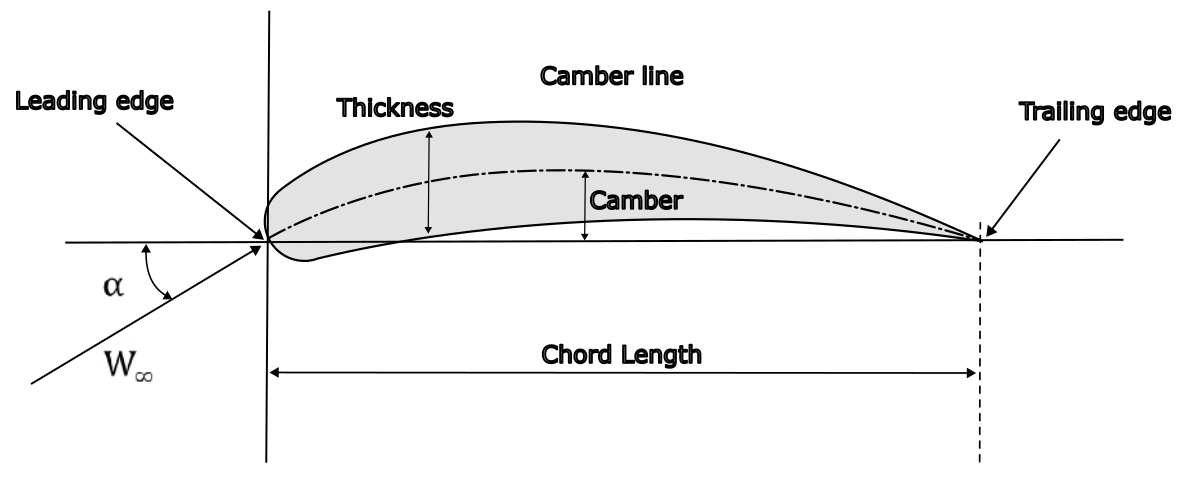
\includegraphics[width=0.8\linewidth]{Figures/Foil2d/Airfoil_basics.png}
    \caption{NACA\,00xx geometrical parameters used throughout the present work.}
    \label{fig:airfoil_geometry}
\end{figure}
 
Three families of two-dimensional coefficients describe the response of an airfoil section to a given relative flow. The lift coefficient $C_L$, the drag coefficient $C_D$ and the minimum-pressure coefficient $C_{p,\min}$ are non-dimensional forms of, respectively, the lift force per unit span, the drag force per unit span, and the lowest static pressure recorded on the section surface. They are defined as
\begin{equation}
C_L \;=\; \frac{L'}{\tfrac{1}{2}\rho V_\infty^{2} c}, \qquad
C_D \;=\; \frac{D'}{\tfrac{1}{2}\rho V_\infty^{2} c}, \qquad
C_{p,\min} \;=\; \frac{p_{\min} - p_\infty}{\tfrac{1}{2}\rho V_\infty^{2}},
\label{eq:CL_CD_Cpmin}
\end{equation}
with $V_\infty$ the freestream relative velocity, $\rho$ the fluid density, $c$ the chord, and $p_\infty$ the freestream static pressure. In a stator cascade these coefficients are reported per radial section and are functions of incidence, geometry and Reynolds number~\cite{Abbott1959}.
 
In the present application, NACA-type symmetric profiles with prescribed thickness ratio and rounded leading edges are used as a base, and the camber line is constructed to match the desired metal angles $\theta_1(r)$ and $\theta_2(r)$ along the span. The link between flow angle, loading and losses is established through the slip-correction methodology established in the project work~\cite{Leonsen2025} and through the cascade analysis developed in Section~\ref{sec:theory_cascade}. The detailed geometric construction implemented in the parametric MATLAB tool used for this thesis is described in Section~\ref{sec:theory_geometric_construction}.
 
% ---------------------------------------------------------------------
\section{Swirl metrics and critical phenomena}
\label{sec:theory_swirl_metrics_def}
 
Quantification of the swirling motion downstream of the RDT and downstream of the guide vanes is one of the central tasks of the post-processing in this thesis. The key quantity is the non-dimensional swirl number $S$. A standard definition expresses it as the ratio between the axial flux of angular momentum and the axial flux of axial momentum times a characteristic radius~\cite{Gupta1984, Vignat2022}:
\begin{equation}
S(z) \;=\; \frac{1}{R}\,\frac{G_\theta(z)}{G_z(z)},
\label{eq:S_def}
\end{equation}
where for an axisymmetric duct of radius $R$
\begin{align}
G_\theta(z) \;&=\; 2\pi\!\int_0^R \rho\, r^2 \, U_\theta(r,z)\,U_z(r,z)\,\mathrm{d}r,
\label{eq:Gtheta}\\
G_z(z) \;&=\; 2\pi\!\int_0^R \rho\, r \, U_z^{2}(r,z)\,\mathrm{d}r.
\label{eq:Gz}
\end{align}
The fundamental design objective of the guide vanes is to reduce $S(z)$ from the high values established by the RDT towards values close to zero at the RPT inlet (Figure~\ref{fig:Verdijk_swirl}). The post-processing in this thesis evaluates $S$ at every analysis plane in the domain (Chapter~\ref{chap:chap4}) so that the spatial development of the swirl can be tracked along the entire path from the RDT through the bend to the RPT inlet.
 
\begin{figure}[h!]
    \centering
    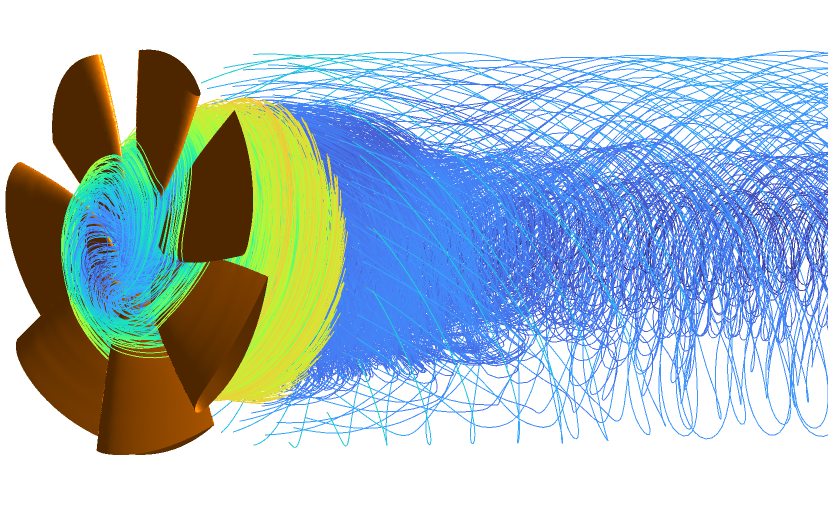
\includegraphics[width=0.75\linewidth]{Figures/Theory/RDT_swirl1.png}
    \caption[Verdijck's swirl pattern]{Swirl pattern downstream of the RDT, taken from Verdijck~\cite{Verdijck2025}.}
    \label{fig:Verdijk_swirl}
\end{figure}
 
\paragraph{Alternative swirl-number definitions.}
Equation~\ref{eq:S_def} is the form most often used in the combustion literature and is the form adopted as the primary metric in this thesis. However, the swirl number is not unique. Vignat et al.~\cite{Vignat2022} show that, when applied to non-uniform velocity profiles or in the presence of significant pressure terms, several formally equivalent definitions can give numerical values that differ by tens of percent. Two variants are particularly relevant here. The \emph{angle-based} swirl indicator
\begin{equation}
\overline{\alpha}(z) \;=\; \arctan\!\Bigl(\overline{U_\theta}^{\,m}(z)/\overline{U_z}^{\,m}(z)\Bigr)
\label{eq:alpha_bar}
\end{equation}
uses the mass-flow-averaged tangential and axial velocity components and has the advantage of being directly interpretable as a flow angle. The \emph{local swirling-strength} indicator $\lambda_{ci}$ identifies vortex cores from the imaginary part of the eigenvalues of the local velocity-gradient tensor and is the field used in CFX as \texttt{Velocity.Swirling Strength}. These two complement Eq.~\ref{eq:S_def}: $\overline{\alpha}$ summarises the bulk swirl orientation, $\lambda_{ci}$ is needed to identify discrete vortex structures such as tip vortices or precessing cores, and $S$ measures the total angular-momentum content of the cross-section. Reporting all three reduces the risk that a particular ranking depends on a particular definition.
 
\paragraph{Critical swirl and vortex breakdown.}
When the swirl ratio exceeds a critical value, swirling pipe flow can develop stagnation zones, wall separation and vortex breakdown~\cite{Rusak2014}. Critical $S$ values reported in the literature cluster around 0.6 for free swirling flows but depend on the specific definition and on the boundary conditions; in confined pipe flow with finite walls the threshold can be higher~\cite{Rusak2014}. Vortex breakdown is associated with large losses and strong unsteadiness, and it is the underlying mechanism behind the rotating vortex rope (RVR) in Francis-turbine draft tubes at off-design~\cite{Brekke2010}. In the present application, a residual $S(z)$ at the RPT inlet plane that is large enough to support breakdown would be unacceptable. The screening therefore checks the residual $S$ values against this threshold.
 
% ---------------------------------------------------------------------
\subsection{Swirl decay in straight pipes}
\label{sec:theory_swirl_decay}
 
In a straight pipe with no swirl-conditioning element, the swirl decays through wall shear and turbulent transport. Experiments by Kitoh~\cite{Kitoh1991} and others show that the decay is approximately exponential and slow relative to typical duct lengths in industrial layouts:
\begin{equation}
S(z) \;\approx\; S(z_0)\,\exp\!\left[\,-\beta\,\frac{z - z_0}{D}\,\right],
\label{eq:S_decay}
\end{equation}
where the decay constant $\beta$ depends weakly on swirl level and Reynolds number and typically takes values $\beta \approx 0.02$--$0.06$ for smooth-walled turbulent flow~\cite{Kitoh1991, Beaubert2016}. The implication is that, for a duct length of a few diameters between the RDT and the RPT, the natural decay alone reduces $S$ only modestly. The decay also adds wall friction, so even the apparent ``benefit'' of letting the swirl decay over a long distance is partly cancelled by additional pressure loss compared with a non-swirling flow at the same Reynolds number. This is the classical motivation for an active swirl-recovery element placed close to the RDT, rather than a long downstream pipe acting as a passive damper~\cite{Andersen2014, Nguyen2024}.
 
\paragraph{Implication for the present geometry.}
The path from the guide-vane trailing-edge plane to the RPT inlet, in the geometry adopted here, is approximately $0.50$~m of straight pipe (cone), then a $90^\circ$ bend, then approximately $1.0$~m of straight pipe in the final inlet section. This is short compared to the decay length expected from Eq.~\ref{eq:S_decay} for the swirl numbers seen at the guide-vane trailing edge. The residual swirl at the RPT inlet is therefore controlled almost entirely by what the guide vanes deliver and not by free decay in the pipe sections. The post-processing in this thesis quantifies this directly by comparing $S$ at the guide-vane trailing edge with $S$ at the bend exit and at the final inlet plane.
 
% ---------------------------------------------------------------------
\section{Cavitation considerations}
\label{sec:theory_cavitation}
 
Cavitation occurs when the local static pressure $p$ in the water falls to or below the vapour pressure $p_v$. Vapour bubbles form in low-pressure regions and collapse again when convected into higher-pressure regions, which can cause erosion, noise, vibration and loss of head and efficiency~\cite{Gulich2010, Plesset1949}. An example of bubble growth and collapse near a wall is shown in Figure~\ref{fig:cavitation_bubbles}.
 
\begin{figure}[h!]
  \centering
  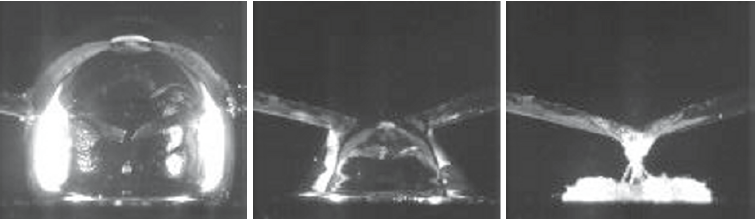
\includegraphics[width=0.8\textwidth]{Figures/Theory/Cavitation_bubbles.png}
  \caption[Cavitation bubbles]{Typical stages of cavitation bubble growth and collapse near a wall, adapted from G\"ulich~\cite{Gulich2010}.}
  \label{fig:cavitation_bubbles}
\end{figure}
 
In pump and pump-turbine applications, the cavitation risk is usually expressed through the available net positive suction head,
\begin{equation}
\mathrm{NPSH}_\mathrm{A} \;=\; \frac{p_{\mathrm{in}} - p_v}{\rho g},
\label{eq:npsha}
\end{equation}
where $p_{\mathrm{in}}$ is the absolute pressure at the machine inlet. For comparison with the machine head $H$, the Thoma cavitation number is
\begin{equation}
\sigma \;=\; \frac{\mathrm{NPSH}_\mathrm{A}}{H} \;=\; \frac{p_{\mathrm{in}} - p_v}{\rho g H},
\label{eq:sigma_thoma}
\end{equation}
and high $\sigma$ corresponds to safe operation, while low $\sigma$ is associated with bubble growth, head loss, efficiency loss and possible erosion~\cite{Franc2007, Gulich2010}.
 
For the NTNU RPT, Kerlefsen reports a required NPSH of approximately $1.3$--$1.4$~m for a net head $H_{\mathrm{net}} \approx 12$~m, giving $\mathrm{NPSH}_\mathrm{R}/H_{\mathrm{net}} \approx 0.11$--$0.12$, with a recommended margin of $20$--$25\,\%$ between available and required NPSH~\cite{Kerlefsen2025}. The Store2Hydro booster is intended to add approximately $H \approx 5$~m of head upstream of the RPT, which is comfortable as long as guide-vane losses are kept moderate. The interpretation in the screening campaign is therefore that any total-pressure loss reduces the available cavitation margin and must be charged against the design.
 
In CFD, cavitation is commonly modelled as a homogeneous mixture of liquid water and water vapour, with mass-transfer rates determined by a Rayleigh--Plesset-based source term. In the present work no cavitation modelling is performed in the screening campaign; the static pressure field is examined for the absence of regions with $p < p_v$, but multiphase modelling is left as future work for the selected configuration.
 
% ---------------------------------------------------------------------
\section{Design requirements for guide vanes}
\label{sec:theory_srv_requirements}
 
Figure~\ref{fig:verdijk_streamlines} and Figure~\ref{fig:shubham_streamlines} show example streamlines downstream of the RDT from earlier and present design work in the Store2Hydro programme. Both flow fields exhibit a strongly swirling wake, but with important differences. Verdijck's simulation~\cite{Verdijck2025} used a rotating fluid domain that extends some distance downstream of the rotor, which produces a visible rotating core with backflow in the centre and may artificially imprint rotation on the wake. The later simulations by Sharma and Djupesland (referenced via~\cite{Leonsen2025}) limit the rotating domain to the blade volume only and give a more representative inflow for the planned guide-vane section. The latter dataset is used as the inlet condition in this thesis.
 
\begin{figure}[h!]
  \centering
  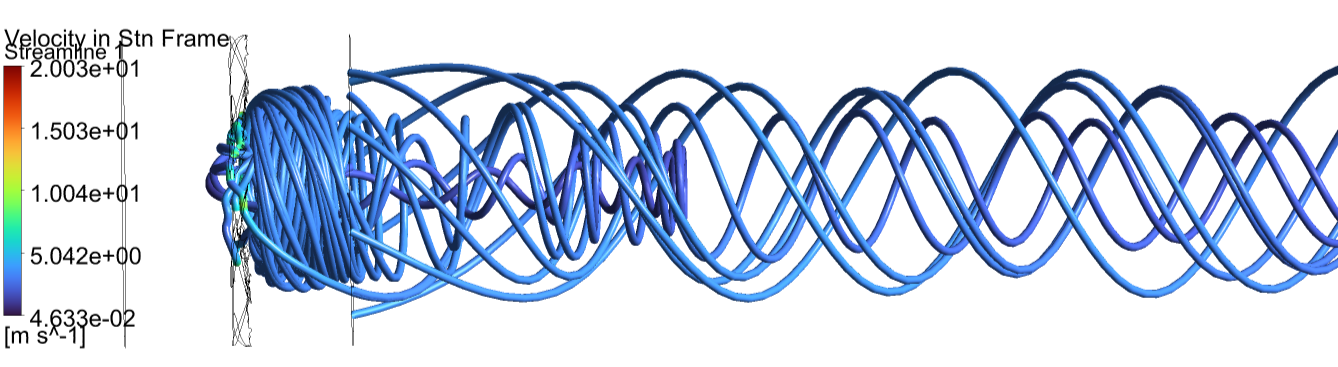
\includegraphics[width=0.83\textwidth]{Figures/Theory/streamlines_edgar1.png}
  \caption[Streamlines downstream, Verdijck]{Streamlines from Verdijck's final RDT design~\cite{Verdijck2025}.}
  \label{fig:verdijk_streamlines}
\end{figure}
 
\begin{figure}[h!]
  \centering
  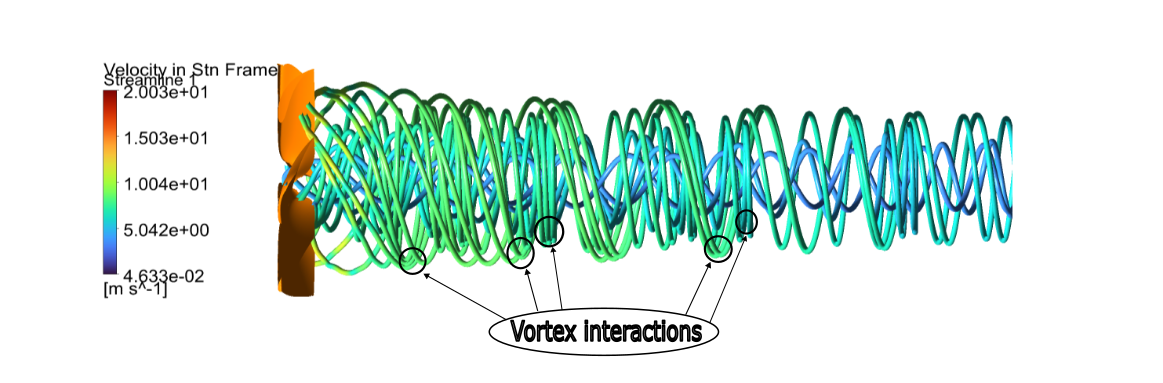
\includegraphics[width=0.99\textwidth]{Figures/Theory/Streamlines_shubham_Ink.png}
  \caption[Streamlines downstream, Sharma and Djupesland]{Streamlines downstream of the RDT from the ongoing work by Sharma and Djupesland. Primary and secondary streamlines merge in vortex interactions across the wake.}
  \label{fig:shubham_streamlines}
\end{figure}
 
The simulations also indicate very large local flow angles in the outer part of the wake. At $r \approx 0.25$~m, the absolute angle between $C_m$ and $C_u$ approaches $80^\circ$--$89^\circ$, meaning the velocity is almost entirely tangential. The guide vanes must therefore be designed to handle extreme inflow angles while still providing controlled turning and acceptable losses.
 
\subsection{Backflow region and the design span}
\label{sec:theory_backflow_span}
 
A central feature of the RDT wake is the central low-momentum or back-flow region. Post-processing of the Sharma--Djupesland simulation indicates that radii up to approximately $r \approx 0.144$~m experience back-flow, with $C_m < 0$ in this region (Figure~\ref{fig:UxUt}). The guide-vane design cannot adapt to this region in any meaningful way because the flow direction is reversed and the vane has no inlet flow with positive momentum to operate on. The guide vanes are therefore designed as a hubless cascade, with the design span restricted to radii with positive meridional flow. In the present geometry this corresponds approximately to $r \in [0.12, 0.25]$~m, i.e.\ $r/R \in [0.48, 1.00]$. The associated flow-angle profile (Figure~\ref{fig:AngleRadius}) varies from approximately $89^\circ$ at the inner design radius to a minimum of about $60^\circ$ at $r \approx 0.225$~m, before increasing slightly again towards the shroud.
 
\begin{figure}[h!]
    \centering
    \includesvg[width=0.75\textwidth]{Figures/SVG/Ux_Ut.svg}
    \caption[Axial and tangential velocity, Sharma's simulation]{Axial and tangential velocity profiles versus radius, $0.25$~m downstream of the Sharma RDT simulation.}
    \label{fig:UxUt}
\end{figure}
\begin{figure}[h!]
    \centering
    \includesvg[width=0.75\textwidth]{Figures/SVG/Angle_radius.svg}
    \caption[Flow-field angle, Sharma's simulation]{Flow-field angle versus radius, $0.25$~m downstream of the Sharma RDT simulation.}
    \label{fig:AngleRadius}
\end{figure}
 
The assumption is that the central recirculation zone carries low momentum flux compared with the main flow at larger radii and will partially mix out downstream before reaching the RPT runner. This assumption is examined in Chapter~\ref{chap:chap5} by comparing the central-region velocity field at the guide-vane outlet plane and at the bend exit.
 
\subsection{Tip-vortex mechanisms}
\label{sec:theory_tip_vortex}
 
When the inflow to the guide vanes has very high swirl, some streamlines hit the leading edge at angles so large that they cannot follow the geometry of the vane. Part of the flow then leaks around the inner free end of the vane into the hubless central region. The pressure difference between the pressure side and the suction side drives this tip-leakage flow, which rolls up into a tip-clearance vortex and creates extra induced vortices in the passage~\cite{You2007}. In the circular hubless cascade considered here, the same type of vortex can appear near the inner ends of the vanes even though the geometry is not a planar two-dimensional cascade. Figure~\ref{fig:Tip_vortex} sketches this mechanism. In the post-processing, this is the structure that the swirling-strength field $\lambda_{ci}$ should pick up most clearly near the inner span of the vanes.
 
\begin{figure}[h!]
  \centering
  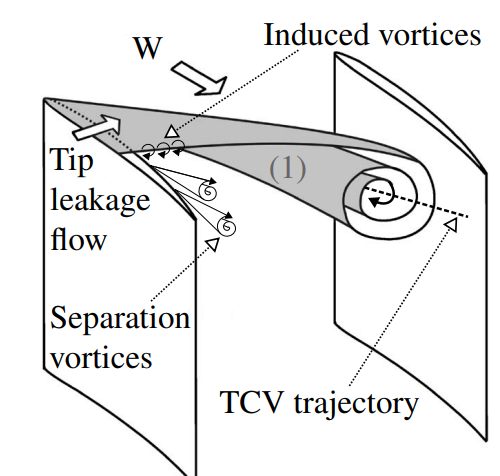
\includegraphics[width=0.40\textwidth]{Figures/Theory/Tip_vortex}
  \caption[Tip-leakage vortex mechanism]{Schematic of tip-leakage flow and the formation of a tip-clearance vortex (TCV), adapted from You et al.~\cite{You2007}.}
  \label{fig:Tip_vortex}
\end{figure}
 
% ---------------------------------------------------------------------
\section{Cascade theory for guide vanes}
\label{sec:theory_cascade}
 
\subsection{Solidity and pitch}
\label{sec:theory_solidity}
 
At each radius $r$, the guide vanes form an axial cascade with pitch
\begin{equation}
s(r) \;=\; \frac{2\pi r}{Z_s},
\label{eq:pitch}
\end{equation}
and local solidity
\begin{equation}
\sigma(r) \;=\; \frac{c(r)}{s(r)},
\label{eq:solidity}
\end{equation}
where $Z_s$ is the vane count and $c(r)$ is the local chord. Solidity controls how much turning the cascade can deliver; high solidity gives more turning per pitch but also more wetted surface, more friction loss and a higher risk of separation between adjacent vanes. The pitch and solidity for the present geometry, evaluated for a fixed chord $c = 0.25$~m and vane counts $Z_s \in \{6, 7, 8, 9\}$, are summarised in Table~\ref{tab:pitch_solidity_design}. The table illustrates a recurring feature of hubless designs: the local solidity rises sharply at the inner radius because the pitch shrinks with $r$, so even a moderate global vane count produces a heavily loaded inner span.
 
\begin{table}[h!]
\centering
\caption[Pitch and solidity for selected vane counts]{Pitch $s(r)$ and solidity $\sigma(r)$ for guide vanes with chord $c = 0.25$~m in a pipe of diameter $D = 0.5$~m, for $Z_s \in \{6,7,8,9\}$ and $r \in [0.12, 0.25]$~m.}
\label{tab:pitch_solidity_design}
\small
\begin{tabular}{c|cc|cc|cc|cc}
\toprule
\textbf{$r$ (m)} & $s$ ($Z{=}6$) & $\sigma$ & $s$ ($Z{=}7$) & $\sigma$ & $s$ ($Z{=}8$) & $\sigma$ & $s$ ($Z{=}9$) & $\sigma$ \\
\midrule
0.12 & 0.1257 & 1.99 & 0.1077 & 2.32 & 0.0942 & 2.65 & 0.0838 & 2.98 \\
0.15 & 0.1571 & 1.59 & 0.1346 & 1.86 & 0.1178 & 2.12 & 0.1047 & 2.39 \\
0.18 & 0.1885 & 1.33 & 0.1616 & 1.55 & 0.1414 & 1.77 & 0.1257 & 1.99 \\
0.21 & 0.2199 & 1.14 & 0.1885 & 1.33 & 0.1649 & 1.52 & 0.1466 & 1.71 \\
0.25 & 0.2618 & 0.95 & 0.2244 & 1.11 & 0.1963 & 1.27 & 0.1745 & 1.43 \\
\bottomrule
\end{tabular}
\end{table}
 
\subsection{Diffusion factor and the de Haller criterion}
\label{sec:theory_diffusion}
 
A standard measure of how heavily a blade row is loaded is the Lieblein diffusion factor~\cite{Lieblein1953}:
\begin{equation}
D_f \;=\; 1 - \frac{V_{\mathrm{out}}}{V_{\mathrm{in}}}
       + \frac{\lvert V_{\theta,\mathrm{out}} - V_{\theta,\mathrm{in}} \rvert}
              {2\,\sigma\, V_{\mathrm{in}}},
\label{eq:Df}
\end{equation}
with $V_{\mathrm{in}}$, $V_{\mathrm{out}}$ the inlet and outlet relative velocities, $V_{\theta,\mathrm{in}}$, $V_{\theta,\mathrm{out}}$ the corresponding tangential components, and $\sigma$ the local solidity. Lieblein recommends $D_f \lesssim 0.6$ to keep the suction-side boundary layer attached. A complementary screening criterion is the de Haller bound on the relative-velocity ratio,
\begin{equation}
\frac{V_{\mathrm{out}}}{V_{\mathrm{in}}} \;\geq\; 0.72,
\label{eq:deHaller}
\end{equation}
which is independent of solidity but cruder than $D_f$. Both criteria are used in the post-processing as descriptive indicators rather than as binary go/no-go limits, because the present application requires turning angles up to $80^\circ$--$90^\circ$ that are well beyond the conventional axial-compressor regime.
 
\subsection{Incidence, deviation and effective turning}
\label{sec:theory_incidence_deviation}
 
Section~\ref{sec:theory_kinematics} introduced the inlet and outlet flow angles $\beta_1(r)$ and $\beta_2(r)$, the metal angles $\theta_1(r)$ and $\theta_2(r)$, the incidence $i(r)$, and the deviation (slip) angle $\delta(r)$. In the cascade view these quantities are used as design constraints:
\begin{itemize}
  \item the leading edge should see a small incidence $i(r)$ at the design point, to avoid early separation and additional loss;
  \item the deviation $\delta(r)$ determines how much of the geometric turning $\theta_1 - \theta_2$ actually appears as flow turning $\beta_1 - \beta_2$;
  \item the effective turning is therefore smaller than the geometric turning, especially for low solidity and high loading.
\end{itemize}
In the present work, the deviation is treated as a fixed correction $\delta_{\mathrm{TE}} = 6^\circ$ added to the trailing-edge metal angle, in line with the recommendation of G\"ulich~\cite{Gulich2010}. The justification is that the slip-database response surface developed in the project work~\cite{Leonsen2025} predicts deviation angles on the order of $10^\circ$--$20^\circ$ at the high-turning conditions seen here, but adopting these large built-in angles rapidly increases the suction-side adverse pressure gradient and tends to promote separation, while a moderate fixed correction captures the bulk of the deviation effect without overloading the cascade. This choice is revisited in Chapter~\ref{chap:chap5} when individual cases are interpreted.
 
% ---------------------------------------------------------------------
\section{Geometric construction of the guide vanes}
\label{sec:theory_geometric_construction}
 
This section describes the geometric construction of each two-dimensional vane section that is produced by the parametric MATLAB tool \texttt{vanedesign\_loft\_export}. The presentation is organised so that each step in the construction can be related to a specific design parameter exposed in the run script \texttt{run\_file\_GV\_DESIGN.m}, which supports later interpretation of the simulation results.
 
\subsection{Chordwise coordinate and clustering}
\label{sec:theory_clustering}
 
A non-dimensional chordwise coordinate $x^* = x/c \in [0, 1]$ is used with cosine clustering near the leading and trailing edges,
\begin{equation}
x^* \;=\; \frac{1 - \cos(\pi t)}{2}, \qquad t \in [0, 1],
\label{eq:cosine_clustering}
\end{equation}
which concentrates points where the surface curvature and the pressure gradient are largest. Cosine clustering is standard practice in airfoil design because it reduces geometric truncation errors at the leading and trailing edges and is preserved when the section is wrapped on a cylindrical or conical surface.
 
\subsection{Cubic camber line and metal-angle matching}
\label{sec:theory_camber}
 
The camber line is a cubic polynomial in $x^*$,
\begin{equation}
\frac{y_c(x^*)}{c} \;=\; A x^{*3} + B x^{*2} + C x^*,
\label{eq:camber_cubic}
\end{equation}
where the coefficients $A$, $B$, $C$ are chosen so that the local slope of $y_c$ at $x^* = 0$ matches the LE metal angle $\theta_1$ and at $x^* = 1$ matches the TE metal angle $\theta_2$, both expressed in a frame aligned with the stagger angle $\zeta$. The cubic form has three free coefficients, which is sufficient to enforce the two slope conditions and one normalisation condition. A cubic polynomial is preferred over a parabola or a circular arc because it allows the LE and TE slopes to be specified independently, which is necessary to match arbitrary inflow and target outflow angles. The choice ties the camber directly to the velocity-triangle requirement and is the reason the design tool can be driven from spanwise inlet data $r$, $C_m(r)$, $C_u(r)$.
 
\subsection{Modified NACA 00xx thickness law}
\label{sec:theory_thickness}
 
The thickness law follows the classical NACA 00-series formula~\cite{Abbott1959}:
\begin{equation}
\frac{t_{\mathrm{base}}(x^*)}{c} \;=\; 5\!\left(0.2969\sqrt{x^*} - 0.1260\,x^* - 0.3516\,x^{*2} + 0.2843\,x^{*3} - 0.1015\,x^{*4}\right),
\label{eq:naca_thickness}
\end{equation}
which produces a symmetric profile with maximum thickness near $x^* \approx 0.30$. Two modifications adapt the law to the guide-vane application. A leading-edge roundness factor $\texttt{LE\_round}$ adjusts the thickness near $x^* = 0$ as
\begin{equation}
t_{\mathrm{LE}}(x^*) \;=\; t_{\mathrm{base}}(x^*)\,\Bigl[\,1 + (\texttt{LE\_round}-1)\,(1-x^*)^2\,\Bigr],
\label{eq:LE_round}
\end{equation}
which thickens the leading edge for $\texttt{LE\_round} > 1$ and thereby reduces sensitivity to off-design incidence. A finite trailing-edge thickness ratio $t_{\mathrm{TE,rel}}$ is added linearly, $t(x^*)/c = a\,t_{\mathrm{LE}}(x^*) + t_{\mathrm{TE,rel}}\,x^*$, with the scale factor $a$ chosen so that $\max_x t(x^*)/c$ matches a prescribed target $(t/c)_{\mathrm{rel}}$. Throughout the present work, $(t/c)_{\mathrm{rel}} = 0.075$ and $\texttt{LE\_round} = 1.2$ are kept fixed, in line with the project work~\cite{Leonsen2025}.
 
\subsection{Stagger angle, lean and sweep}
\label{sec:theory_stagger_lean_sweep}
 
The stagger angle $\zeta(r)$ orients the chord line relative to the axial direction. It is determined by the choice of metal angles $\theta_1(r)$ and $\theta_2(r)$ together with the geometric definition that places the chord line at the average of the LE and TE positions in the rotated frame. In addition to the stagger, the design tool exposes two spanwise stacking parameters: \emph{lean} $\texttt{lean\_amp}$ tilts the section in the tangential direction along the span, and \emph{sweep} $\texttt{sweep\_amp}$ shifts the section in the axial direction along the span. Lean and sweep are used in modern axial design to control radial pressure gradients and to mitigate secondary flows~\cite{Schnoes2018}, but in the screening campaign of this thesis they are held at zero so that the chord and solidity factors can be isolated. Lean and sweep are listed as candidates for a second-stage refinement campaign in Chapter~\ref{chap:chap7}.
 
\subsection{Cylindrical or conical wrapping}
\label{sec:theory_wrapping}
 
The two-dimensional sections are stacked along the span and wrapped on either a cylindrical surface of radius $r$ or a conical surface with radius varying linearly with the axial coordinate~\cite{Leonsen2025}. The azimuthal coordinate of each section point is computed from the tangential coordinate and a global trailing-edge anchoring angle. The trailing edges of all sections can be anchored to a common azimuth, $\phi_{\mathrm{TE,global}}$, which produces a straight TE line in the axial--azimuthal plane and supports a clean axial through-flow when the residual swirl is small. In the present work, cylindrical wrapping is used because the guide-vane domain has constant duct diameter and there is no need to wrap on a cone. The TE-anchored option is enabled, which produces all sections aligned at the same azimuth at the trailing edge.
 
\subsection{Constant chord versus constant solidity}
\label{sec:theory_const_chord_const_sol}
 
The two design strategies adopted in the screening campaign are exposed by the boolean flag \texttt{use\_sigma} in the design tool:
\begin{itemize}
  \item \textbf{Constant chord (CC).} The chord $c$ is a single constant value, identical at every radius. The solidity $\sigma(r) = c\,Z_s/(2\pi r)$ then decreases hyperbolically with radius, so the loading per pitch is concentrated near the inner span and decreases towards the shroud.
  \item \textbf{Constant solidity (CS).} The chord is set as $c(r) = \sigma_{\mathrm{target}}\,s(r)$ with $\sigma_{\mathrm{target}}$ fixed, so the solidity is uniform in radius and the chord scales linearly with $r$. The loading is more even radially, but the wetted surface and the friction loss are larger because the outer span receives the longest chord.
\end{itemize}
The two strategies are not equivalent, and the screening campaign is constructed precisely to compare them at matched levels of loading. In the case-naming convention used throughout this thesis, a case label of the form \texttt{CC\_400\_8} denotes a constant-chord design with shroud chord $c = 400$~mm and $Z_s = 8$ vanes, while \texttt{CS\_400\_8} denotes a constant-solidity design with the same shroud chord but with chord scaling linearly inwards.
 
% ---------------------------------------------------------------------
\section{Secondary flow and Dean vortices in 90$^\circ$ bends}
\label{sec:theory_dean_bend}
 
The geometry adopted for the screening campaign includes a $90^\circ$ bend between the cone and the final inlet section. This element is not passive. When fluid passes through a curved duct, the centripetal acceleration $V^2/R_c$ requires a radial pressure gradient across the cross-section. The velocity, however, is not uniform: it is reduced near the wall by the boundary layer and is largest in the core of the duct. The local centripetal acceleration is therefore not uniform across the section, and the cross-stream pressure gradient cannot balance it everywhere simultaneously. The fluid responds by establishing a pair of counter-rotating secondary cells in the cross-stream plane: the \emph{Dean vortices}~\cite{Dean1927}.
 
\subsection{The Dean number and bend regimes}
\label{sec:theory_dean_number}
 
The strength of the Dean vortices scales with the dimensionless Dean number
\begin{equation}
\mathrm{De} \;=\; \mathrm{Re}\,\sqrt{\frac{D_h}{2\,R_c}},
\label{eq:dean}
\end{equation}
where $D_h$ is the hydraulic diameter of the duct and $R_c$ is the radius of curvature of the bend centreline. For the present geometry the duct diameter at the bend is approximately $D = 0.4$~m and the bend curvature radius is on the order of $R_c \approx 0.3$--$0.4$~m. With Reynolds numbers around $\mathrm{Re} \sim 10^6$ in the duct, the Dean number is well into the turbulent regime where the Dean cells are fully developed and may further interact with the upstream-imposed swirl. Three regimes are commonly distinguished. For $\mathrm{De} \lesssim 100$, the bend secondary flow is laminar and weak. For intermediate Dean numbers, instabilities and additional secondary cells (D\"ottner cells) emerge. For high Reynolds numbers, the secondary motion is fully turbulent and is dominated by two large counter-rotating Dean cells, with additional small-scale features near the inner radius where separation is most likely.
 
\subsection{Interaction with upstream swirl}
\label{sec:theory_swirl_bend_interaction}
 
When the upstream flow already carries swirl, the Dean cells and the swirl interact non-trivially. If the upstream swirl rotates in the same sense as one of the two Dean cells, that cell is amplified and the opposite cell is suppressed; if the upstream swirl rotates in the opposite sense, the partition is reversed. The post-bend axial-velocity profile is therefore generally asymmetric in a way that depends on the \emph{sign} of the residual swirl, not only on its magnitude. Liu and Vanierschot~\cite{LiuVanierschot2021} review this regime and document that the asymmetry persists for several diameters downstream of the bend exit. Escue and Cui~\cite{EscueCui2010} demonstrate that the SST $k$--$\omega$ model captures the bulk structure of swirling pipe flow but tends to underpredict turbulence anisotropy under strong rotation, which is one of the recognised limitations when interpreting RANS results in this regime.
 
The implication for the present thesis is that:
\begin{enumerate}
  \item the guide-vane performance must be evaluated not only at the trailing-edge plane (where the design tool has direct geometric leverage) but also at planes downstream of the bend, because swirl--bend interaction changes the effective ranking;
  \item the sign of the residual swirl is a relevant design parameter even if the screening matrix focuses primarily on chord-strategy and vane count;
  \item asymmetry of the axial-velocity profile at the RPT inlet plane, not just its mean magnitude, must be reported.
\end{enumerate}
 
\subsection{Inner-radius separation in the bend}
\label{sec:theory_bend_separation}
 
A further bend-related effect is separation on the inner radius of the bend, where the adverse pressure gradient is strongest. Jenssen~\cite{Jenssen2020} reported this effect in the original RPT draft-tube geometry and used it to motivate the placement of a velocity-profile boundary condition downstream of the bend rather than upstream. In the present configuration the same inner-radius separation may occur and is likely to be more severe when the upstream swirl reinforces the inner-side pressure gradient. The screening campaign reports the static-pressure field along the bend centreline and the wall-streamline pattern on the inner radius for the shortlisted cases.
 
% ---------------------------------------------------------------------
\section{Turbulence modelling and numerical limitations}
\label{sec:theory_turbulence}
 
The simulations in this thesis use a Reynolds-averaged formulation with the SST $k$--$\omega$ turbulence model of Menter~\cite{Menter1994}. The SST model blends the standard $k$--$\omega$ model in the near-wall region, where it is robust under adverse pressure gradients, with a $k$--$\varepsilon$ formulation in the outer flow. It is the de-facto standard for hydraulic turbomachinery in industrial CFD and has been validated extensively in pump, turbine and stator applications. The known limitations relevant to the present work are summarised here and revisited where the corresponding limitation is in play.
 
\paragraph{Anisotropy under strong rotation.} Two-equation eddy-viscosity models assume an isotropic eddy viscosity and cannot represent the full Reynolds-stress anisotropy under strong rotation or strongly curved streamlines. In swirling pipe flow this leads to underprediction of secondary kinetic energy in the cross-stream plane and to a slightly diffused tangential-velocity profile compared with experimental data~\cite{EscueCui2010}.
 
\paragraph{Streamline curvature and bend secondary flow.} The Dean vortices in the $90^\circ$ bend are produced by the same streamline-curvature mechanism that two-equation eddy-viscosity models tend to underpredict. The bulk Dean structure is captured, but the magnitude of the secondary-velocity components and the location of inner-radius separation can be sensitive to mesh resolution and to the specific blending of the SST coefficients. The interpretation in Chapter~\ref{chap:chap5} is therefore qualitative when comparing absolute Dean strengths between configurations and quantitative when comparing relative changes between similar configurations.
 
\paragraph{Transition modelling.} Transition is not modelled in the SST formulation used here. The Reynolds numbers in the present application are large enough that the boundary layers on the guide vanes are turbulent everywhere, except possibly in a small region close to the leading edge of the inner span where the local chord-Reynolds number is lowest. The expected effect of neglected transition is a small underestimation of leading-edge loss, which is the same direction for all configurations and therefore does not affect the comparative ranking.
 
\paragraph{Steady RANS for the screening.} The 24-case screening uses steady RANS, which means that the inherent unsteadiness associated with rotor--stator interaction, with vortex shedding from the trailing edge of the guide vanes, and with any precessing vortex core that may develop downstream is not resolved. A separate transient simulation of the baseline configuration is performed to address the rotor--stator interaction question (Chapter~\ref{chap:chap4}, Sections~\ref{sec:rsi-thesis}--\ref{sec:spec-coherence}). Full transient screening of all 24 configurations is not feasible within the time-frame and is left as future work.

\section{Rotor--stator interaction and pressure pulsations}
\label{sec:rsi}
 
In the compact RDT--GV--duct configuration considered in
this thesis, the rotating RDT blades and the stationary GV
ring are separated by a relatively small axial distance. The flow
through the GV is therefore not steady in a strict sense even
at the nominal operating point. Two mechanisms produce unsteady
loading on the GV and a corresponding pressure pulsation field
in the duct \cite{Brekke2015, Arndt1990}:
\begin{enumerate}
  \item \emph{Potential interaction.} The pressure field attached to
        each rotor blade convects past the stationary vanes. It
        produces a pressure fluctuation that decays exponentially
        with axial distance but can be significant when the axial
        gap is a fraction of a blade chord.
  \item \emph{Viscous (wake) interaction.} Each rotor blade sheds a
        velocity-deficit wake. When such a wake is chopped by a
        stationary vane, the local angle of attack changes
        momentarily and produces an impulsive change in vane loading.
\end{enumerate}
Both mechanisms are periodic in the rotor reference frame at the
rotor frequency~$f_n$, and in the stator reference frame at the
blade passing frequency~$f_{\mathrm{BPF}}$ defined below. They are
the main source of deterministic unsteadiness in the present
configuration.
 
\subsection{Rotor frequency and blade passing frequency}
\label{sec:rsi-bpf}
 
With rotor rotational speed $n$~(rpm), the rotor frequency
is
\begin{equation}
    f_n \;=\; \frac{n}{60}. \label{eq:fn}
\end{equation}
A single stationary vane observes $Z_r$ rotor blades passing in each
rotor revolution. The fundamental excitation frequency seen by a
single GV is therefore the \emph{blade passing
frequency}~\cite{Brekke2015}
\begin{equation}
    f_{\mathrm{BPF}} \;=\; Z_r\, f_n. \label{eq:fbpf}
\end{equation}
A single rotor blade sees $Z_s$ stationary vanes per rotor revolution
and therefore experiences a periodic loading at the \emph{vane
passing frequency}
\begin{equation}
    f_{\mathrm{VPF}} \;=\; Z_s\, f_n. \label{eq:fvpf}
\end{equation}
In the special case $Z_r = Z_s$ the two frequencies coincide,
$f_{\mathrm{BPF}} = f_{\mathrm{VPF}}$. Higher harmonics
$k f_{\mathrm{BPF}}$, $k=2,3,\dots$ are typically present because
the actual pulse shape is not sinusoidal; their amplitude decreases
with $k$ but can remain non-negligible for the second and third
harmonic if the wake is
narrow~\cite{Egusquiza2006,Rodriguez2007}.
 
\subsection{Tyler--Sofrin modal decomposition}
\label{sec:rsi-tyler}
 
The classical analysis by Tyler and Sofrin~\cite{Tyler1962} for an
annular rotor--stator stage shows that the unsteady pressure field
downstream of the stator can be written as a sum of circumferential
modes
\begin{equation}
    p'(r,\theta,z,t) \;=\; \sum_{k=1}^{\infty}\sum_{j=-\infty}^{\infty}
      \hat{p}_{k,j}(r,z)\,
      \exp\!\left[\, i\bigl(m_{k,j}\,\theta - k\,Z_r\,\Omega\,t\bigr)\,\right],
    \label{eq:tyler_sofrin_expansion}
\end{equation}
where $\Omega = 2\pi f_n$ and the circumferential mode order is
\begin{equation}
    m_{k,j} \;=\; k\,Z_r - j\,Z_s, \qquad k,j \in \mathbb{Z}.
    \label{eq:tyler_sofrin}
\end{equation}
Each combination $(k,j)$ corresponds to a pressure pattern that
rotates around the axis with phase speed $k\,Z_r\,\Omega/m_{k,j}$ and
oscillates at frequency $k f_{\mathrm{BPF}}$ at a fixed point in the
stator frame. The mode order $m_{k,j}$ determines how the pulsation
couples with the surrounding duct: an $m=0$ pattern is axisymmetric
and propagates as a plane wave, whereas patterns with $|m|\geq 1$
are spinning modes whose upstream or downstream propagation depends
on whether the frequency is above or below the cut-off frequency of
the corresponding duct mode~\cite{Morse1968}.
 
For the fundamental BPF harmonic $k=1$ the lowest-order spatial mode
is
\begin{equation}
    m_{\min} \;=\; \min_{j\in\mathbb{Z}} \bigl| Z_r - j\,Z_s \bigr|.
    \label{eq:mmin}
\end{equation}
Three cases are of particular relevance:
\begin{itemize}
  \item If $Z_r = Z_s$, Eq.~\eqref{eq:mmin} gives $m_{\min}=0$ with
        $k=j=1$. The lowest-order mode at $f_{\mathrm{BPF}}$ is the
        \emph{axisymmetric breathing mode}: all $Z_s$ vanes are
        loaded synchronously and in phase. The pressure field is a
        plane wave that propagates along the duct without a cut-off,
        and the integrated axial force on the GV ring adds
        coherently at $f_{\mathrm{BPF}}$.
  \item If $\gcd(Z_r,Z_s)=1$ (coprime), the minimum mode order is at
        least $|Z_r - Z_s|$ and typically $m_{\min} \geq 1$. The net
        axial force on the ring approaches zero by cancellation
        around the circumference. The remaining loading appears as a
        rotating radial force on the rotor.
  \item If $Z_r = Z_s = 7$, the baseline configuration in this
        thesis, the breathing mode $m=0$ is unavoidable in principle.
        Whether it actually dominates the pulsation field in practice
        depends on how closely the true wake pattern of the RDT
        satisfies the $Z_r$-fold azimuthal symmetry that the
        Tyler--Sofrin argument assumes.
\end{itemize}
It is therefore an established design guideline in axial
turbomachinery to choose $Z_r$ and $Z_s$ such that low-order spatial
modes are avoided at the harmonics of concern, especially when
structural or acoustic natural frequencies lie close to
$f_{\mathrm{BPF}}$~\cite{Brekke2015,Egusquiza2006,Tanaka2011}. For
reversible pump-turbines in particular,
reference~\cite{Nduwayezu2021} reports that the vaneless-space
pressure pulsation amplitude depends explicitly on the runner blade
number, which supports treating $Z_s$ as a system-level design
variable and not only as a hydraulic one.
 
\subsection{Structural and acoustic resonance}
\label{sec:rsi-resonance}
 
Unsteady blade forcing becomes critical when an excitation frequency
in Eq.~\eqref{eq:tyler_sofrin_expansion} approaches a structural or
acoustic natural frequency of the system. Two coupling categories
are typically considered~\cite{Egusquiza2006,Tanaka2011}.
 
\paragraph{Structural resonance.} The GV blade, the GV
ring, the RDT blades and the supporting structure each possess
a discrete set of natural frequencies $\{f_k^s\}$. A resonance
condition occurs when an excitation frequency $k\,f_{\mathrm{BPF}}$
or $k\,f_{\mathrm{VPF}}$ matches one of the $f_k^s$, \emph{and} the
spatial mode order of the excitation is compatible with the
deformation mode shape. A breathing ($m=0$) pressure pulsation will
efficiently excite axial bending or piston-like modes, while a
spinning ($m\geq 1$) pulsation will efficiently excite diametrical
modes with the matching nodal diameter count.
 
The GV blade operates in water and therefore has a strong
added-mass effect. Wet natural frequencies are generally 25--40\,\%
lower than the corresponding dry values~\cite{Tanaka2011}. For a
compact hydraulic GV of the dimensions considered here, the
lowest wet bending mode is expected to lie well above 100~Hz, but
this should be verified by a separate modal analysis before a final
GV design is committed to~\cite{Valentin2015}.
 
\paragraph{Acoustic resonance.} In confined liquid systems, standing
pressure waves can build up if an excitation frequency coincides with
an acoustic mode of the duct. Acoustic resonance is most commonly
associated with the $m=0$ component of $f_{\mathrm{BPF}}$ because
the plane-wave mode propagates without cut-off~\cite{Nicolet2007}.
 
\subsection{Practical magnitudes and resonance thresholds}
\label{sec:rsi-magnitudes}
 
Whether an unsteady loading constitutes a practical design concern
is decided by the \emph{amplitude} of the pulsation relative to the
mean loading, not by its spectral location alone. Brekke's monograph
on hydraulic turbines~\cite{Brekke2015,Brekke2010} and the IEC~60193
standard provide the following order-of-magnitude guidelines:
\begin{itemize}
  \item Normalised pressure pulsation amplitudes
        $\tilde{p}_{E} = A_p / (\rho g H)$ below approximately
        $1\,\%$ at the blade passing frequency are generally
        acceptable for continuous operation.
  \item Values in the range $1$--$3\,\%$ indicate significant
        rotor-stator interaction and warrant careful design review
        and structural fatigue assessment.
  \item Values above $3$--$5\,\%$ are indicative of resonance or of
        operation close to a hydraulic instability, and usually
        require design modification.
\end{itemize}
Equivalent thresholds for the cyclic force amplitude on a single
vane are not uniformly tabulated, but reported case studies on
Francis-type machines show that fluctuation amplitudes below
$0.5\,\%$ of the mean vane load at $f_{\mathrm{BPF}}$ are typical in
safely operating units~\cite{Egusquiza2006}. These reference values
are used as diagnostic thresholds in the interpretation of the
CFD results in Chapter~\ref{ch:results}.
 
\subsection{Relation to the present thesis}
\label{sec:rsi-thesis}
 
The choice $Z_r = Z_s = 7$ of the baseline configuration places the
fundamental spatial mode at $m_{\min} = 0$ at the frequency
$f_{\mathrm{BPF}} = 7\,f_n$. The theoretical expectation is that
this configuration is \emph{a priori} unfavourable compared with
configurations using $Z_s \in \{5,6,8,9\}$, for which
$m_{\min} \geq 1$ and the net axial force on the GV ring at
$f_{\mathrm{BPF}}$ would cancel to leading order.
 
The design matrix used in the simulation campaign therefore includes
$Z_s \in \{5,6,7\}$, so that this hypothesis can be tested directly
in the actual RDT--GV configuration and not only argued
from classical theory. Whether the breathing mode actually
manifests at a significant amplitude depends on the degree of
$Z_r$-fold azimuthal symmetry of the incoming RDT wake and on
the spanwise matching between rotor and stator, both of which are
imperfect in practice. A diagnostic for the effective weight of the
$m=0$ mode in the computed pulsation field is introduced in
Section~\ref{sec:spec-coherence}.


\section{Flow fundamentals and turbomachinery kinematics}
Reuse alot




\subsection{Governing equations, coordinate systems, and reference frames}
\label{sec:theory_kinematics}

The flow between the rim-driven thruster (RDT) and the reversible pump-turbine (RPT) is treated as an incompressible turbulent flow and is modelled in the present work using a Reynolds-averaged formulation. For steady single-phase flow of water, the governing equations are the continuity equation and the Reynolds-averaged momentum equation. In compact vector form, these are written as

\begin{equation}
\nabla \cdot \mathbf{u} = 0,
\end{equation}

\begin{equation}
\rho \left( \mathbf{u} \cdot \nabla \mathbf{u} \right)
=
-\nabla p
+ \mu \nabla^2 \mathbf{u}
- \rho \nabla \cdot \overline{\mathbf{u}'\mathbf{u}'}.
\end{equation}

Here, \(\mathbf{u}\) is the mean velocity vector, \(p\) is the mean static pressure, \(\rho\) is the fluid density, \(\mu\) is the dynamic viscosity, and \(-\rho \overline{\mathbf{u}'\mathbf{u}'}\) is the Reynolds-stress tensor that represents the effect of unresolved turbulent fluctuations. In a Reynolds-averaged Navier--Stokes framework, these stresses must be closed through a turbulence model. This formulation is appropriate for the present study because the main objective is to compare mean-flow quantities such as total-pressure loss, swirl reduction, and downstream flow quality, rather than to resolve the full unsteady turbulent spectrum \cite{Pope2000}.

A cylindrical coordinate system is a natural choice for the present geometry because the duct, the RDT wake, and the guide-vane annulus are all organised around a common centreline. The flow is therefore described in cylindrical coordinates \((r,\theta,z)\), where \(z\) is the axial direction from the RDT towards the RPT, \(r\) is the radial coordinate measured from the duct centreline, and \(\theta\) is the circumferential coordinate. The absolute velocity vector \(\vec{C}\) is written as

\begin{equation}
\vec{C}(r,\theta,z)
=
C_r(r,\theta,z)\,\hat{e}_r
+
C_\theta(r,\theta,z)\,\hat{e}_\theta
+
C_z(r,\theta,z)\,\hat{e}_z,
\end{equation}

where \(C_r\) is the radial component, \(C_\theta\) the tangential or swirl component, and \(C_z\) the axial component.

\paragraph{Notation.}
In the CFD post-processing, the velocity components are often reported as \(U_x\) and \(U_t\). In the cascade and turbomachinery notation used for the guide-vane design, the same components are written as meridional and tangential absolute velocity, such that

\begin{equation}
C_m \equiv U_x \equiv C_z,
\qquad
C_u \equiv U_t \equiv C_\theta.
\end{equation}

Throughout this thesis, the symbols \(C_m\) and \(C_u\) are used as the preferred notation for the mean axial and tangential velocity components. Software-specific labels such as \texttt{Velocity.Axial}, \texttt{Velocity.Circumferential}, \(U_x\), and \(U_t\) are only used when referring explicitly to CFD monitor expressions or post-processing variables.

Downstream of the RDT, the flow resembles a confined swirling pipe flow. Experimental and analytical studies of such flows show that the radial velocity is often small compared with the axial and tangential components, and that the swirl decays gradually downstream under the action of wall friction and turbulent transport \cite{Kitoh1991}. For this reason, many reduced descriptions of developed swirling pipe flow use a base state where the radial velocity is neglected. In the present work, the RDT outlet and the guide-vane design inlet are therefore described with the approximation

\begin{equation}
C_r \approx 0,
\end{equation}

so that the flow is primarily characterised by the axial and tangential components,

\begin{equation}
C_m \equiv C_z,
\end{equation}

\begin{equation}
C_u \equiv C_\theta.
\end{equation}

This assumption should be interpreted as a design-level simplification rather than a full description of the resolved flow. It is useful when the incoming RDT wake is reduced to spanwise profiles of \(C_m(r)\) and \(C_u(r)\) for guide-vane design, but it does not imply that the full flow is axisymmetric or free of radial transport. Once the flow enters the guide-vane passage, the individual vanes introduce local blockage, turning, wakes, and end-wall effects that vary around the circumference. Further downstream, the conical section and the \(90^\circ\) bend introduce additional asymmetry and secondary-flow motion. The CFD problem must therefore still be treated as fully three-dimensional even though the design input is reduced to spanwise profiles.

In turbomachinery, it is convenient to describe the flow using velocity triangles that relate the absolute velocity \(\vec{C}\), the relative velocity \(\vec{W}\) seen by a rotating blade row, and the blade speed \(\vec{u}\). The relative velocity is written as

\begin{equation}
\vec{W} = \vec{C} - \vec{u},
\end{equation}

where the local blade speed at radius \(r\) is

\begin{equation}
u(r)=\omega r,
\end{equation}

with \(\omega\) denoting the angular velocity of the rotor \cite{DixonHall2014}. This distinction between absolute and relative velocity is fundamental in rotor rows such as the RDT or the RPT runner, where blade loading is naturally interpreted in the rotating frame.

For the guide vanes considered in the present thesis, the situation is simpler because the vane row is stationary. The guide-vane passage is therefore solved in a stationary frame of reference. In that sense, the absolute and relative frames are physically identical for the guide-vane domain itself. Nevertheless, the relative-velocity notation remains useful because it provides a direct connection to classical cascade quantities such as inlet angle, outlet angle, metal angle, incidence, and deviation. In rotating CFD domains, a solver may instead employ a rotating frame of reference, in which the momentum equations include the appropriate Coriolis and centrifugal source terms. In ANSYS CFX, these source terms are introduced automatically when a rotating frame is defined for the domain \cite{AnsysCFXRotatingFrames2024}.

The local kinematics of the flow are represented by velocity triangles. Figure~\ref{fig:vel_triangles_overview} illustrates the velocity triangles at the RDT outlet and at the guide-vane inlet and outlet. At each radius, the incoming and outgoing velocities are decomposed into axial and tangential components, and the corresponding flow angles are defined relative to the axial direction. The absolute flow angle at the guide-vane inlet is defined as

\begin{equation}
\alpha_2(r) = \tan^{-1}\left(\frac{C_{u2}(r)}{C_{m2}(r)}\right).
\end{equation}

The corresponding metal angles at the leading and trailing edges are denoted by \(\theta_1(r)\) and \(\theta_2(r)\), and the stagger angle \(\zeta(r)\) defines the orientation of the chord line relative to the axial direction. The relative flow angles upstream and downstream of the vane are denoted by \(\beta_1(r)\) and \(\beta_2(r)\), respectively. The incidence angle at the leading edge is then written as

\begin{equation}
i(r) = \beta_1(r) - \theta_1(r),
\end{equation}

and a central design requirement is to keep \(i\) small in order to avoid leading-edge separation and the associated increase in loss \cite{DixonHall2014}.

\paragraph{Choice of flow angle for stationary guide-vane design.}
A central distinction in the design of the present guide vanes is that
they are stationary components. In the absolute frame in which the vane row is evaluated, the relevant inflow direction at the leading edge is fully described by the absolute flow angle $\alpha(r)$ defined in \eqref{eq:alpha_definition}, since $\vec{W}\equiv \vec{C}$ when the local blade speed is zero. The relative flow angle
$\beta(r)=\arctan(W_u/C_m)$ is therefore not used to set the
guide-vane metal angles in this thesis; it is reported in
Section~\ref{sec:methods_rdt_velocity_triangles} only as a kinematic
descriptor of the upstream rotor wake. In contrast, the design of the
upstream RDT~\cite{Verdijck2025} is naturally formulated in the
relative frame of the rotor blades and uses $\beta$, while the
guide-vane generator of Leonsen~\cite{Leonsen2025} expects spanwise
$(C_m,\,C_u)$ profiles and computes the absolute angle internally as
$\alpha = \arctan(C_u/C_m)$. The two angle conventions are consistent
once the appropriate frame of reference is identified.

The assumptions introduced in this section define the modelling scope used throughout the thesis. The upstream wake is reduced to spanwise distributions of meridional and tangential velocity at a selected plane downstream of the RDT. These profiles are then used to generate candidate guide-vane geometries through a blade-element type design procedure. The subsequent CFD simulations resolve the three-dimensional mean flow through the vane row and the connected duct sections. This provides a practical framework for screening guide-vane concepts while retaining the dominant physical mechanisms that govern swirl recovery, hydraulic loss, and downstream inlet quality.



\clearpage % Keep this at the end of the chapter